\section{System Design}
\label{sec:design}

\begin{figure*}[t]
\centering
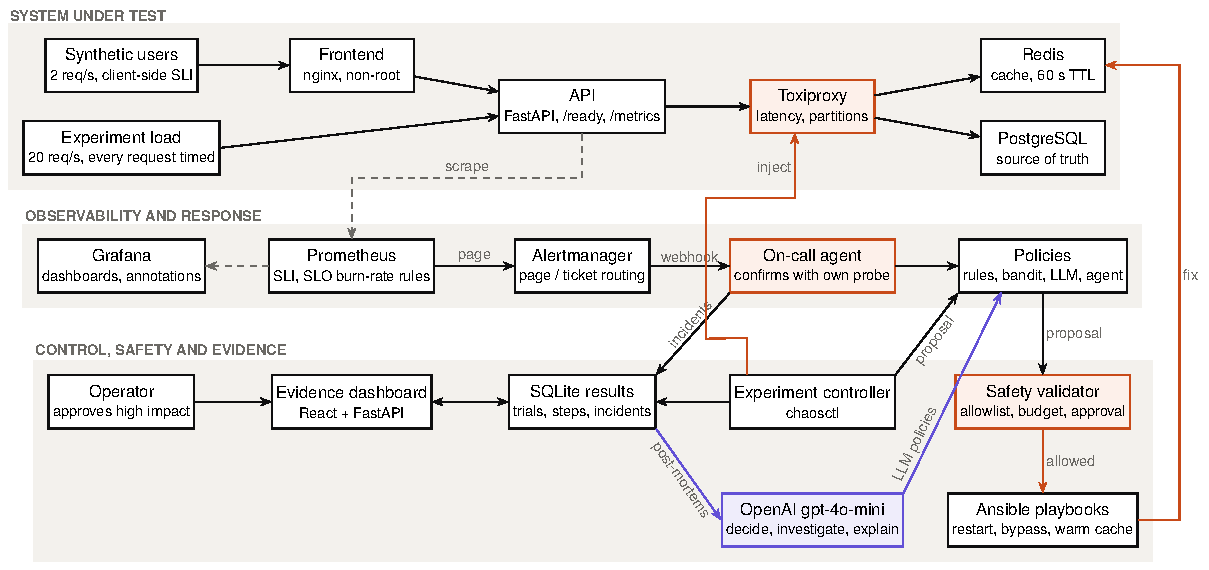
\includegraphics[width=\textwidth]{architecture.pdf}
\caption{\sys{} architecture. Faults enter through Toxiproxy (network) and Docker (process kills);
fixes enter through Ansible playbooks after the safety validator. The on-call agent is woken only by
Alertmanager; experiments are driven by the controller. All decisions and outcomes are stored in
SQLite and shown in the evidence dashboard; gpt-4o-mini is the only external service.}
\label{fig:arch}
\end{figure*}

Fig.~\ref{fig:arch} shows the three layers of \sys{}: the system under test, observability and
response, and control, safety and evidence. All components run as containers in one Docker Compose
project per lab; overlay files add host ports locally, an HTTPS proxy on servers, or a tunnel for
sharing. Each lab has a unique project name, so the CI pipeline can start isolated labs next to a
developer's lab on the same Docker host.

\subsection{System under test}
The target is a deliberately small shop: an nginx frontend, a FastAPI service and a catalogue of
1{,}000 items read with the cache-aside pattern from Redis (60\,s TTL) in front of PostgreSQL. Redis
calls time out after 500\,ms; database access uses a pool of 10 connections with 2\,s timeouts. A
Redis error yields HTTP~503 unless a \emph{cache-bypass} flag routes reads to PostgreSQL. The API
exposes liveness (\texttt{/health}), readiness with dependency probe latencies (\texttt{/ready}),
Prometheus metrics, and two administrative endpoints used by recovery actions. The API reaches both
data stores \emph{through Toxiproxy}~\cite{toxiproxy}, so latency and partitions can be injected
without touching the stores themselves.

\subsection{Faults}
Table~\ref{tab:faults} lists the seven faults. Five are used for training and design; two are
\emph{held out} and were run only after all policies were frozen. The partition is designed to look
like \act{redis\_down} to an observer while making a restart useless; the compound fault makes
cache bypass harmful.

\begin{table}[t]
\caption{Fault scenarios}
\label{tab:faults}
\centering
\small
\begin{tabular}{@{}lp{4.1cm}c@{}}
\toprule
Fault & Injection & Set \\
\midrule
\act{redis\_down} & kill the Redis container & train \\
\act{redis\_latency} & +800\,ms on Redis traffic ($>$ 500\,ms timeout) & train \\
\act{postgres\_latency} & +400\,ms on PostgreSQL traffic & train \\
\act{postgres\_down} & kill the PostgreSQL container & train \\
\act{api\_crash} & kill the API container & train \\
\midrule
\act{redis\_partition} & disable the Redis proxy (container healthy) & held out \\
\act{redis\_down\_slow\_db} & kill Redis and +400\,ms on PostgreSQL & held out \\
\bottomrule
\end{tabular}
\end{table}

\subsection{Load and recovery measurement}
\label{sec:measure}
Prometheus scrapes every 5\,s, too coarse for recoveries of 1--2\,s. During experiments an
\emph{open-model} load generator therefore sends 20 requests/s for random items regardless of
response times (a closed model would silently send less traffic during an outage) and records
the send time, completion time and status of every request (2\,s timeout).

Let requests be grouped into 1-second windows $w_i$ by send time after injection at $t_0$. A window
is \emph{healthy} if
\begin{equation}
\frac{|\{r \in w_i : r \text{ ok}\}|}{|w_i|} \ge 0.99 \;\wedge\; p_{95}(w_i) \le 300\,\text{ms},
\end{equation}
and empty windows are unhealthy. The service has \emph{recovered} once $k=5$ consecutive healthy
windows follow the first unhealthy window. To resolve recovery below window granularity, the
recovery time is the send time of the first request after the last \emph{bad} request (failed or
slower than 300\,ms) preceding that healthy run, minus $t_0$. A trial whose 10\,s pre-injection
baseline is unhealthy is marked invalid and excluded. These definitions are implemented in one
unit-tested module.

\subsection{Remediation loop and actions}
After detection (the last completed 1\,s window is unhealthy), the controller runs a loop modelled
on incident response: observe symptoms, ask the policy for an action, check it with the safety
validator, execute it, and wait up to 20\,s for three healthy seconds. If the service healed, the
step succeeded; otherwise the loop observes again, up to three executed actions per incident.
Policies see only \emph{symptoms}: error rate and p95 over the last second, whether the API answers,
and Redis/PostgreSQL reachability and probe latency from \texttt{/ready}; never the fault's name.

Actions are Ansible playbooks (Table~\ref{tab:actions}). Restarts locate containers by Compose
labels, refuse services outside an allowlist (\act{api}, \act{redis}, \act{postgres},
\act{frontend}), restart them and wait for readiness; \act{cache\_bypass} and \act{warm\_cache} call
the API's administrative endpoints (warming uses a dedicated database connection so that it does
not queue behind an exhausted pool).

\begin{table}[t]
\caption{Recovery actions, safety impact and reward cost}
\label{tab:actions}
\centering
\scriptsize
\setlength{\tabcolsep}{3.5pt}
\begin{tabular}{@{}lp{3.35cm}cc@{}}
\toprule
Action & Effect & Impact & Cost \\
\midrule
\act{restart\_redis} & restart Redis, await readiness & medium & 0.05 \\
\act{restart\_postgres} & restart PostgreSQL & high & 0.20 \\
\act{restart\_api} & restart the API & medium & 0.10 \\
\act{cache\_bypass} & serve reads from PostgreSQL & low & 0.05 \\
\act{warm\_cache} & load all items into Redis (10\,min) & low & 0.02 \\
\bottomrule
\end{tabular}
\end{table}

\subsection{Safety shield}
\label{sec:safety}
Every proposal, from every policy, is checked in order against a declarative policy file; the first
failing rule blocks it and the reason is recorded: (1)~the lab's project name must match an approved
pattern; (2)~the action must be on the allowlist; (3)~no action may repeat within an incident,
which prevents restart loops; (4)~at most three actions may execute per incident; (5)~high-impact
actions need approval. Approval is \emph{auto} (logged) in the isolated experiment lab, \emph{human}
in on-call mode, or \emph{deny}. The playbooks enforce their own service allowlist as an independent
second layer. A red-team policy proposes destructive and non-allowlisted actions on purpose.

\subsection{Policies}
\label{sec:policies}
\textbf{Runbook.} Restart whatever looks broken, then restart the API; a common operational default.

\textbf{Expert heuristic.} Rules written after studying the training results (e.g.\ PostgreSQL
probe $>$200\,ms $\Rightarrow$ \act{warm\_cache}; Redis unreachable $\Rightarrow$ \act{cache\_bypass}).

\textbf{LinUCB bandit.} The context $x \in \mathbb{R}^8$ contains a bias, binary indicators for API
down, Redis unreachable and PostgreSQL unreachable, log-scaled probe latencies
$\ell(m)=\min(\log(1+m)/\log(2001),1)$ for both stores, the error rate, and $\ell(p_{95})$. Each
executed step yields the reward
\begin{equation}
r = \max\!\left(0,\, 1 - \frac{t_{\text{heal}}}{20\,\text{s}}\right) - c(a),
\end{equation}
with $r=-c(a)$ if the step never healed and $c(a)$ the safety cost in Table~\ref{tab:actions}. For
each action $a$, disjoint LinUCB~\cite{li2010linucb} maintains $A_a = I + \sum x x^\top$ and
$b_a = \sum r\,x$, predicts $\hat\theta_a^\top x$ with $\hat\theta_a = A_a^{-1} b_a$, and scores
$\hat\theta_a^\top x + \alpha\sqrt{x^\top A_a^{-1} x}$ with $\alpha=0.5$. The model is trained
offline on logged steps of training faults only (an assertion rejects held-out data) and acts
greedily among actions not yet tried in the incident.

\textbf{LLM.} gpt-4o-mini~\cite{openai2024mini} receives the symptoms, the allowed actions with
descriptions, and what has already run or been blocked, and returns JSON with an action and a
one-sentence reason (temperature~0).

\textbf{LLM agent.} The same model and prompt, plus five tools: an instant PromQL query, the last
two minutes of a shop container's log (repeated lines collapsed), container states, the readiness
check, and \texttt{decide(hypothesis, action, reason)}. The agent must call at least one
investigation tool before \texttt{decide} is offered and is forced to decide after five. The fault
injector is invisible to all tools. Every call and result is stored as an auditable trail.

\textbf{Ablation variants.} Both LLM policies also exist with one added paragraph of generic SRE
guidance (restarts only fix crashed or hung processes, not slow or unreachable networks, and lose
warm state; check down vs.\ slow; prefer the least disruptive action; consider side effects). It
names no fault and no action.

\subsection{On-call mode}
\label{sec:oncall}
\begin{figure}[t]
\centering
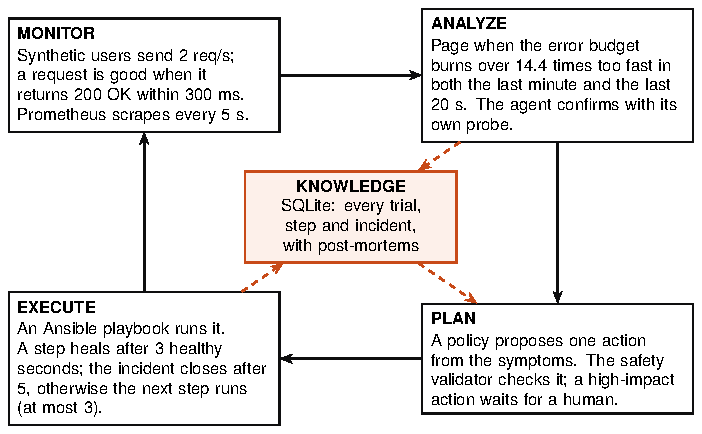
\includegraphics[width=\columnwidth]{loop.pdf}
\caption{The on-call loop mapped onto MAPE-K~\cite{kephart2003vision}.}
\label{fig:loop}
\end{figure}

Experiments know when and what they inject. On-call mode removes that knowledge (Fig.~\ref{fig:loop}).
A synthetic-user service sends 2 requests/s and counts each request as \emph{good} (200 within
300\,ms), \emph{slow} or \emph{error}; the SLI is measured at the client because the API cannot count
requests it never receives. The SLO is 99\% good requests, so the error budget is $\epsilon=0.01$.
With $\rho_w$ the bad-request ratio over window $w$, the burn rate is $\beta_w=\rho_w/\epsilon$.
Following the SRE Workbook~\cite{beyer2018workbook}, scaled from hours to lab time, Prometheus pages
when
\begin{equation}
\beta_{1\,\text{min}} > 14.4 \;\wedge\; \beta_{20\,\text{s}} > 14.4,
\end{equation}
raises a ticket when $\beta_{1\,\text{h}} > 3 \wedge \beta_{10\,\text{min}} > 3$, and raises a ticket
if the synthetic traffic itself is not scraped for 30\,s. These rules are unit-tested with
\texttt{promtool}: an outage pages and stops paging after recovery, a 5\,s blip does not page, and
slow responses burn budget like errors.

Alertmanager delivers pages to the agent's webhook (group wait 1\,s, repeat every minute) and
inhibits the slow-burn ticket while the page fires. On a page, the agent (i)~stands down if
autopilot is off or an experiment holds the shared lab lock; (ii)~sends its own probe traffic
(10 requests/s for 4\,s) and dismisses the page as stale if three consecutive seconds are healthy,
because windowed alerts lag behind reality; (iii)~opens an incident and runs the remediation loop
with a shield in \emph{human} approval mode: a high-impact proposal creates an approval request that
an operator approves or denies in the dashboard, only the first decision counts, and with no
decision in 60\,s the action is not run; (iv)~closes the incident only on sustained recovery (five
healthy windows), otherwise escalates to a human without retrying; an escalation closes
automatically once the service is healthy; and (v)~asks gpt-4o-mini for a post-mortem from the
incident record. The agent runs in its own container and never reads the chaos log, so every
incident is detected from symptoms alone. On the chaos side, the dashboard can inject a chosen or
random fault unannounced, a chaos monkey can inject random faults at jittered intervals, and every
injected fault is rolled back after five minutes. A scorecard matches each logged fault to the first
incident opened within ten minutes and reports time to alert, to engagement and to recovery.

\subsection{Evidence and generative AI}
All trials, steps (symptoms, verdict, timing, reward, the LLM's reason, the agent's trail), incidents,
approvals and faults are stored in SQLite on a shared volume. A React dashboard presents the fixed-action
matrix, policy rankings, the learning curve, per-incident timelines, the on-call console and the safety
log. gpt-4o-mini writes post-mortems and answers free-form questions strictly from the measured data;
it is never a source of numbers.

\subsection{CI/CD pipeline and DevSecOps}
\label{sec:cicd}
\begin{figure*}[t]
\centering
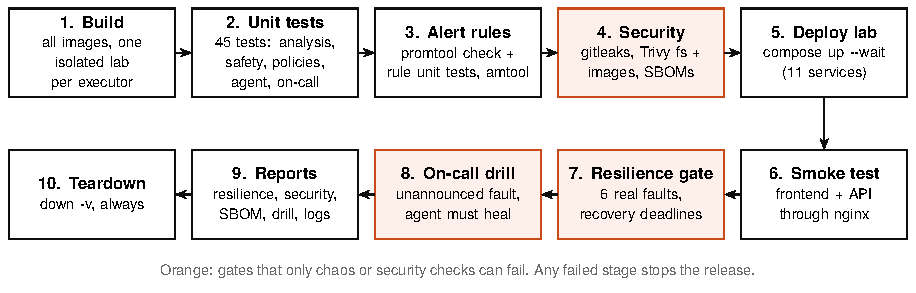
\includegraphics[width=0.86\textwidth]{pipeline.pdf}
\caption{The Jenkins pipeline. Every stage is a gate; the security scan, the resilience gate and the
on-call drill are the stages that only chaos or security findings can fail.}
\label{fig:pipeline}
\end{figure*}

A Jenkins multibranch job, defined as code, builds every branch (Fig.~\ref{fig:pipeline}). Each build
starts its own lab without host ports and tears it down afterwards. Besides unit tests and a smoke
test, four stages are specific to \sys{}: \emph{alert rules} (\texttt{promtool} and \texttt{amtool}
checks and rule unit tests); a \emph{security scan} with gitleaks over the working tree and the whole
git history, Trivy over pinned Python and npm dependencies (including build-time dependencies) and
Dockerfiles, and Trivy over every built image with a CycloneDX SBOM archived per image; a
\emph{resilience gate} that runs six real faults with a fixed action each and fails if recovery
exceeds a deadline (10--20\,s, about twice the locally measured median); and an \emph{on-call
drill} that kills Redis without notice and fails unless the agent heals it within 120\,s. Sources
reach scanners through standard input rather than bind mounts, because Jenkins drives the host's
Docker engine. A production overlay places Caddy in front of the dashboard as the only public entry
point (automatic HTTPS, bcrypt login, security headers), and an Ansible playbook provisions a fresh
Ubuntu server in one command; a Cloudflare tunnel shares a laptop lab behind the same login.
